% Options for packages loaded elsewhere
\PassOptionsToPackage{unicode}{hyperref}
\PassOptionsToPackage{hyphens}{url}
%
\documentclass[
  12pt,
]{article}
\usepackage{lmodern}
\usepackage{amssymb,amsmath}
\usepackage{ifxetex,ifluatex}
\ifnum 0\ifxetex 1\fi\ifluatex 1\fi=0 % if pdftex
  \usepackage[T1]{fontenc}
  \usepackage[utf8]{inputenc}
  \usepackage{textcomp} % provide euro and other symbols
\else % if luatex or xetex
  \usepackage{unicode-math}
  \defaultfontfeatures{Scale=MatchLowercase}
  \defaultfontfeatures[\rmfamily]{Ligatures=TeX,Scale=1}
\fi
% Use upquote if available, for straight quotes in verbatim environments
\IfFileExists{upquote.sty}{\usepackage{upquote}}{}
\IfFileExists{microtype.sty}{% use microtype if available
  \usepackage[]{microtype}
  \UseMicrotypeSet[protrusion]{basicmath} % disable protrusion for tt fonts
}{}
\makeatletter
\@ifundefined{KOMAClassName}{% if non-KOMA class
  \IfFileExists{parskip.sty}{%
    \usepackage{parskip}
  }{% else
    \setlength{\parindent}{0pt}
    \setlength{\parskip}{6pt plus 2pt minus 1pt}}
}{% if KOMA class
  \KOMAoptions{parskip=half}}
\makeatother
\usepackage{xcolor}
\IfFileExists{xurl.sty}{\usepackage{xurl}}{} % add URL line breaks if available
\IfFileExists{bookmark.sty}{\usepackage{bookmark}}{\usepackage{hyperref}}
\hypersetup{
  pdftitle={How does colic affect a horse's life?},
  hidelinks,
  pdfcreator={LaTeX via pandoc}}
\urlstyle{same} % disable monospaced font for URLs
\usepackage[margin=1in]{geometry}
\usepackage{longtable,booktabs}
% Correct order of tables after \paragraph or \subparagraph
\usepackage{etoolbox}
\makeatletter
\patchcmd\longtable{\par}{\if@noskipsec\mbox{}\fi\par}{}{}
\makeatother
% Allow footnotes in longtable head/foot
\IfFileExists{footnotehyper.sty}{\usepackage{footnotehyper}}{\usepackage{footnote}}
\makesavenoteenv{longtable}
\usepackage{graphicx,grffile}
\makeatletter
\def\maxwidth{\ifdim\Gin@nat@width>\linewidth\linewidth\else\Gin@nat@width\fi}
\def\maxheight{\ifdim\Gin@nat@height>\textheight\textheight\else\Gin@nat@height\fi}
\makeatother
% Scale images if necessary, so that they will not overflow the page
% margins by default, and it is still possible to overwrite the defaults
% using explicit options in \includegraphics[width, height, ...]{}
\setkeys{Gin}{width=\maxwidth,height=\maxheight,keepaspectratio}
% Set default figure placement to htbp
\makeatletter
\def\fps@figure{htbp}
\makeatother
\setlength{\emergencystretch}{3em} % prevent overfull lines
\providecommand{\tightlist}{%
  \setlength{\itemsep}{0pt}\setlength{\parskip}{0pt}}
\setcounter{secnumdepth}{-\maxdimen} % remove section numbering
\usepackage{wrapfig}
\usepackage{lipsum}

\title{How does colic affect a horse's life?}
\usepackage{etoolbox}
\makeatletter
\providecommand{\subtitle}[1]{% add subtitle to \maketitle
  \apptocmd{\@title}{\par {\large #1 \par}}{}{}
}
\makeatother
\subtitle{Executive Summary - STAT 405: Final Project}
\author{David Sun, Elizabeth Morales, Jaehee Jeong\\
Sarah Heuschele, Tyler Chun, Yolanda Jin\\
~\\
Team Name: i need a \textless/br\textgreater{}}
\date{6/1/2021}

\begin{document}
\maketitle

{
\setcounter{tocdepth}{2}
\tableofcontents
}
The research report focuses on the benefits of colic surgery for horses
that are admitted into the hospital for abdominal issues. Colic surgery
is used to treat issues that affect the longevity of a horse, most
commonly used to address issues within the gastrointestinal tract. The
data gave us a look into 299 hospital cases of horses that were admitted
due to poor health, and of those horses which lived, died, or were
euthanized. The data also provided an indicator to whether the horse
received surgery or not. Our analysis focused on looking at the horses
admitted and their outcome. From there, we wanted to explore the key
characteristics of the horse's condition to determine if the outcome
could have been different had they received surgery, especially the
horses that had symptoms related to Colic Surgery.")

\begin{figure}
\centering
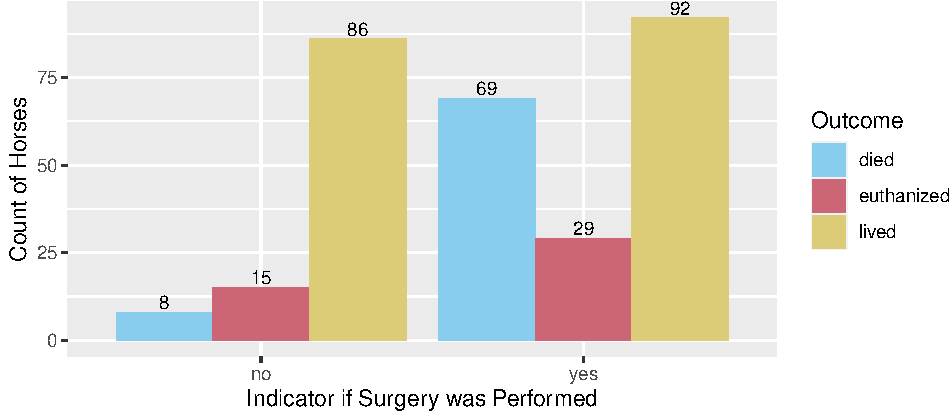
\includegraphics{Final-Project---Executive-Summary_files/figure-latex/unnamed-chunk-4-1.pdf}
\caption{Horse Outcome vs Surgery Performed}
\end{figure}

This analysis is proved useful in determining if colic surgery can be
beneficial in saving a horse's life when admitted into the hospital. Our
initial hypothesis was that the increase in surgeries to treat
gastrointestinal tract complications in horses would lead to an increase
in the number of horses that lived.

With the data given, we explored the different components of a horse's
health, focusing primarily on their gastrointestinal tract. A few of the
key factors were the horse's protein levels, pH levels and rectal
temperature.

From our initial analysis, we found that while the number of horses that
lived did not change much between horses who had surgery and those who
did not, the number of horse that died after surgery grew by about 3
times the amount of those without surgery.

Based on this discovery, we wanted to explore the correlation what
brought the horse to the hospital, if they received surgery, and how
that affected the outcome. The data provided insight on whether the
horse entered the hospital due to something that was deemed ``worthy of
surgery.'' We used this in conjunction with if the horse actually
received surgery to expand on the hypothesis that horses that need
surgery, and receive surgery, are more likely to live.

\begin{longtable}[]{@{}llrrr@{}}
\toprule
Was it Surgical? & Did They Have Surgery & Died & Euthanized &
Lived\tabularnewline
\midrule
\endhead
no & no & 6 & 5 & 75\tabularnewline
no & yes & 2 & 10 & 11\tabularnewline
yes & no & 13 & 12 & 8\tabularnewline
yes & yes & 56 & 17 & 84\tabularnewline
\bottomrule
\end{longtable}

\textbf{Conclusions}

\begin{itemize}
\tightlist
\item
  Adult horses have higher survival rate than young horses
\item
  Horses with multiple treatments had a 20\% higher chance of being
  euthanized or dying
\item
  Those who lived have three times higher proportions (around 60\%) of
  normal and warm temperatures than those who died or euthanized
  (18\textasciitilde20\%)
\item
  About 70\% of lived horses had normal peripheral pulse and about 70\%
  of died or euthanized horses had problematic peripheral pulses
\item
  The distribution for lived horses had more stable rectal temperatures
  than the other two groups.
\item
  About 60\% of the lived horses had normal circulation when about
  20\textasciitilde25\% of the died or euthanized horses had normal
  circulation
\item
  About 70\% of the horses without surgery survived when horses who had
  surgery, around 53\% lived, and 32\% died
\end{itemize}

\end{document}
